\documentclass{standalone}

\usepackage{tikz}
\usetikzlibrary{trees}

\def\yhat{\hat{y}}

\begin{document}
  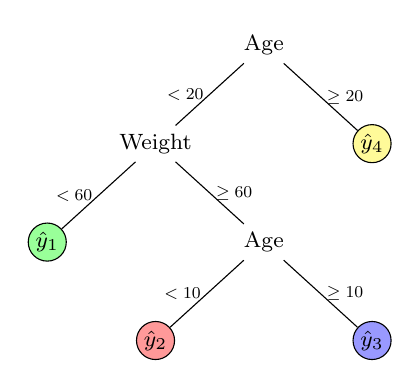
\begin{tikzpicture}[
      level distance=1.25cm,
      sibling distance=2.75cm
    ]
    \footnotesize
    \node {Age}
      child {
        node {Weight}
        child {
          node[circle,draw,fill=green!40,inner sep=1pt] {$\yhat_1$} edge from parent node[left,scale=0.75] {$< 60$}
        }
        child {
          node {Age}
          child {
            node[circle,draw,fill=red!40,inner sep=1pt] {$\yhat_2$} edge from parent node[left,scale=0.75] {$< 10$}
          }
          child {
            node[circle,draw,fill=blue!40,inner sep=1pt] {$\yhat_3$} edge from parent node[right,scale=0.75] {$\geq 10$}
          }
          edge from parent node[right,scale=0.75] {$\geq 60$}
        }
        edge from parent node[left,scale=0.75] {$< 20$}
      }
      child {
        node[circle,draw,fill=yellow!40,inner sep=1pt] {$\yhat_4$} edge from parent node[right,scale=0.75] {$\geq 20$}
      };
  \end{tikzpicture}
\end{document}
